\section{\label{sub:reduxoffline}Redux Offline}
%``Persistenter Redux store für \it{reasonaboutable}\tm ~Offline First Anwendungen``. \\
Redux Offline kann nur zusammen mit Redux verwendet werden~\cite{redux-req}.
Deswegen ist für die Verwendung von Redux Offline die Implementierung von Redux eine Voraussetzung.
%
% Redux
%
% Alles beginnt mit dem Aufruf von \tt{store.dispatch(action)} von jeder beliebigen Stelle in der Anwendung. Die Aktion die beschreibt was passiert heißt \tt{toggleEdit} und sieht im Beispiel des Ansichtswechsels aus wie in Zeile drei bis fünf.\\
% Der \tt{Store} ruft nun den Reducer auf
\sub{\label{chap:redux}Redux}
% Redux ist eine JavaScript Bibliothek, die Probleme im Zusammenhang mit dem Zustand, dem sogenannten \gls{App}state einer Anwendung, löst.
Redux ist eine Bibliothek zur Zustandsverwaltung in JavaScript--Anwendungen.
Es gibt einen zentralen Ort, in dem der Zustand der App gespeichert ist, auf den von jeder Komponente aus zugegriffen werden kann.
Dieser Ort wird Store genannt und jede Applikation hat genau einen davon. 
Als einzige Informationsquelle für den Store als zentralen Speicher dienen Aktionen. 
Aktionen beschreiben was passiert und senden Daten von der Anwendung an den Store.
Eine Aktion könnte beispielsweise die Information beinhalten, dass es eine Aktualisierung gab und auf welchem Objekt diese Aktualisierung stattgefunden hat.
Der dritte wichtige Bestandteil von Redux sind die Reducer. Sie spezifizieren, wie der \gls{App}state, der Status der Applikation, sich als Reaktion auf die Aktionen ändert~\cite{redux}.\\
Der Datenfluss in der Reduxarchitektur ist unidirektional. Zur Veranschaulichung wird anhand der folgenden Abbildung der Redux Datenfluss beschrieben.
%
\begin{figure}[H]
  \centering
  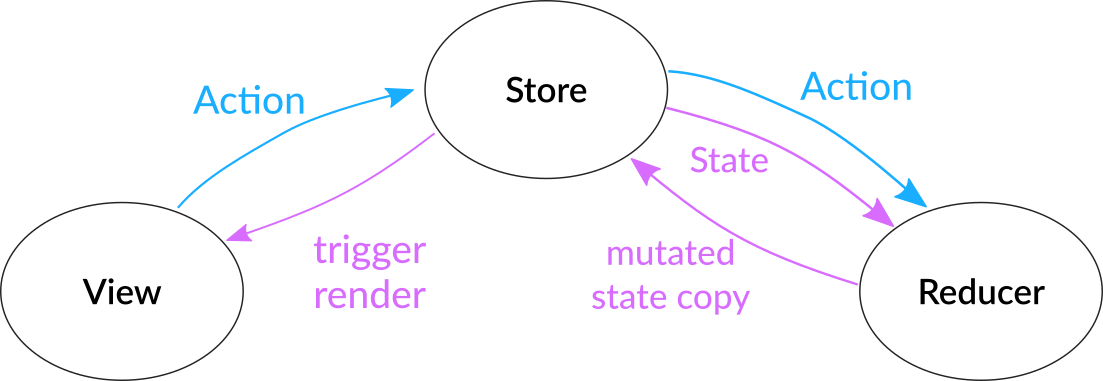
\includegraphics[width=0.8\textwidth]{redux-flow}
  \grayRule
  \caption{Redux Datenfluss}
  \label{fig:rdx-dataflow}
\end{figure}
% 
Zuerst sendet die View eine Aktion an den Store. Dieser empfängt die Aktion und schickt sie zusammen mit dem Applikationsstatus an den Reducer.
Der Reducer erstellt eine Kopie des Status, verändert diese und schickt sie wieder zurück an den Store.
Der Store ersetzt nun den alten mit dem neuen Status und löst ein erneutes Rendern der View aus ~\cite{reduxflow}.
% 
% Redux Offline
% 
\sub{Redux Offline}
Redux Offline erweitert Redux um einen persistenten Store mit Offline First--Technologie und ist kompatibel mit allen *View Frameworks wie React\footnote{JavaScript Bibliothek: \url{https://reactjs.org/}}, Vue\footnote{JavaScript Framework: \url{https://vuejs.org/}}, oder Angular\footnote{JavaScript Framework: \url{https://www.angular.io}}~\cite{redux-offline-compabilaty}.
Es umfasst unter anderem netzwerkfähige \gls{API}-Aufrufe, das Persistieren des Zustands der Anwendung, das Speichern von Aktionen, die Behandlung von Fehlern und erneute Versuche, die Verbindung wieder herzustellen.
Redux Offline verspricht nicht, die Webanwendung komplett offlinefähig zu machen.
Um \gls{Assets} zwischenzuspeichern, muss zusätzlich ein Service Worker implementiert sein ~\cite{redux-offline-gh}.\\
Die Idee hinter Redux Offline ist, dass der Redux Store die Datenbank ersetzt~\cite{redux-offline}.
Bei jeder Änderung wird der Redux Store auf dem Datenträger gespeichert, und bei jedem Start automatisch neugeladen.
Für das Speichern der Daten in einer lokalen Datenbank wird intern \hyperref[sub:reduxpersist]{Redux Persist} verwendet.\\\\
%
%
Eine mit Redux Offline erstellte Anwendung funktioniert ohne weitere Codeimplementierung lokal offline, da das Lesen und Schreiben aus der lokalen Datenbank bereits eingebunden ist.
Damit die Anwendung auch offline funktioniert, wenn sie über das Netzwerk kommuniziert, müssen einige Anpassungen vorgenommen werden.
Sämtliche Daten der Anwendung können nur über Aktionen manipuliert werden. 
Alle netzwerkgebundenen Aktionen werden in einer storeinternen \gls{Queue} gespeichert und müssen mit einem Metaattribut dekoriert werden, um offline arbeiten zu können. Durch die Metaattribute weiß die Anwendung, was vor der eigentlichen Ausführung der Aktion und was danach zu tun ist. 
Es gibt drei Metadaten, die Redux Offline interpretieren kann:\\
\tt{meta.offline.effect} - Die initiale Aktion wird ausgeführt. Hier kann eine URL angegeben werden, die Redux Offline anfragen soll.\\
\tt{meta.offline.commit} - Hier wird die Aktion definiert, die ausgeführt wird sobald die Netzwerkanfrage erfolgreich ist.\\
\tt{meta.offline.rollback} - Hier kann die Aktion angegeben werden, die bei permanent fehlgeschlagener Internetverbindung oder wenn der Server einen Serverfehler zurückgibt, gefeuert wird.
Dann fügt Redux Offline dem \gls{App}state automatisch ein \tt{offline} Objekt hinzu. Dort wird unter anderem ein Array namens \tt{outbox} verwaltet.
Dieses Array repräsentiert die \gls{Queue}. Hier werden die Aktionen inklusive Metadaten gespeichert, um bei bestehender Internetverbindung abgearbeitet zu werden~\cite{redux-offline-docs}.
Die von Jani Eväkallio erstellte Grafik \ref{fig:redux-offline} veranschaulicht die oben erklärte Architektur.
%
\begin{figure}[h]
  \centering
  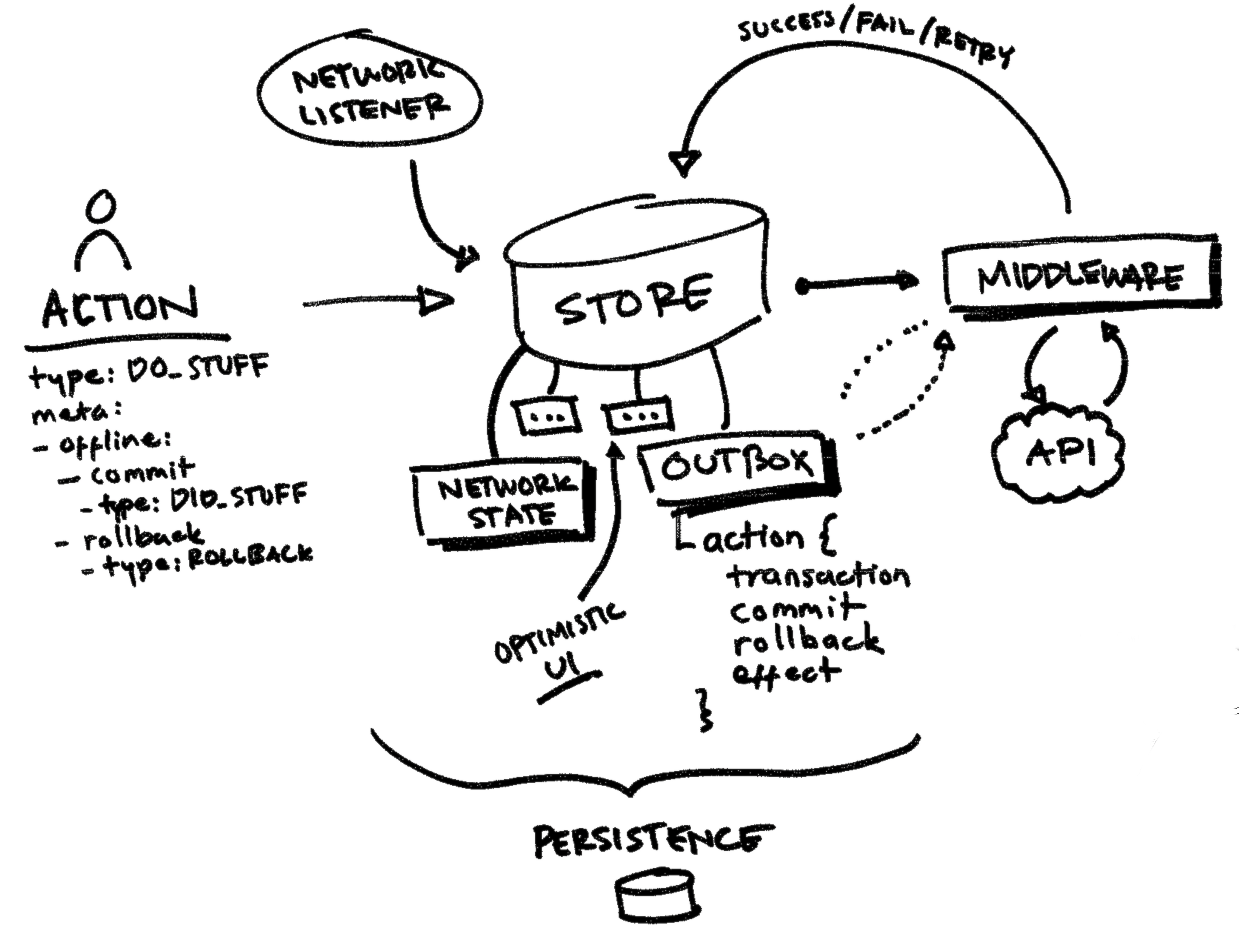
\includegraphics[width=0.8\textwidth]{redux-offline-new}
  \grayRule
  \caption[Redux Offline]{Redux Offline--Architektur -- Quelle:~\cite{redux-offline}}
  \label{fig:redux-offline}
\end{figure}
%
Links ist eine Aktion zu sehen, die ''Zeug'' machen möchte. Sie hat ein Metaattribut das weitere Aktionen definiert, eine Aktion für den Erfolg und eine für den Fehlschlag von `DO\_STUFF`.
In der Mitte ist der Store zu sehen.
Der Store kennt den Netzwerkstatus und umfasst die \gls{Queue} namens \tt{outbox} in dem Aktionen mitsamt ihrer Metafelder gespeichert werden.
Rechts befindet sich das \gls{API}, das über die \gls{Middleware} mit dem Store kommuniziert.\\
Wird die Aktion 'DO\_STUFF' gefeuert gelangt sie in den Store, damit dieser den \gls{App}state aktualisieren kann und wird ersteinmal in der \gls{Queue} gespeichert.
Ist die Anwendung online, wird sie sofort abgearbeitet.
Wenn nicht, wird sie erst einmal in der \gls{Queue} gespeichert bis die Anwendung wieder eine Verbindung zum Internet hat.
% \subsub{Konflikte}
%
% redux persist
%
\sub{\label{sub:reduxpersist}Redux Persist}
Redux Persist ist eine Bibliothek, die als Wrapper für den Redux Store funktioniert.
Mit Redux Persist wird der State automatisch lokal, per default im Local Storage, gespeichert~\cite{redux-persist}.
Es kann konfiguriert werden, wo die Daten gespeichert werden.
Hierfür gibt es diverse Möglichkeiten, wie zum Beispiel im Session Storage, per localForage oder in Dateisystemen~\cite{redux-persist-gh}.
LocalForage ist eine Bibliothek, mit der Daten in der IndexedDB oder in WebSQL gespeichert werden können.
Wenn der Browser die Speichermöglichkeiten nicht unterstützt, wird der Local Storage genommen~\cite{localforage}.\\
Es ist auch möglich einen eigenen Speicher zu konfigurieren.
Die einzige Voraussetzung hierfür ist, das \gls{API} muss die Standardmethoden \tt{setItem}, \tt{getItem} und \tt{removeItem} implementieren und Promises unterstützen~\cite{redux-persist-gh}.
%
% redux optimist
%
% \sub{redux-optimist}